\chapter{Compiler Overview}\label{Chp:CompilerOverview}
When creating a compiler there is two basic ways of compilers one can create, a multi-pass compiler or a single-pass compiler.
Each have their advantages and disadvantages however the most significant difference is that in a single-pass compiler, as the name suggests, only one pass is done.
This highly limits the information available to the compiler and this decreases the odds of creating efficient programs, which is not wished for in \gls{gamble}.
As such this compiler will be a multi-pass compiler, such a compiler can be divided into phases.
In this chapter the different phases of the compiler and their goals and tasks will be presented, to give an overview for the chapters to come.

The compiler for \gls{gamble} is separated into three phases: syntax analysis, contextual analysis and code generation.
\myref{fig:phases} shows a state diagram of the phases of the compiler.
Syntax analysis and contextual analysis transforms the source code into an intermediate representation, and verifies the source code according to the specified syntax from the \acrshort{cfg}, and also for type and scope checking.
The choice of language for writing the compiler falls upon Java 1.8, which is used in the language and compiler course.
When making a compiler an object-oriented language simplifies many tasks, because of encapsulation, polymorphism and inheritance. 
The paradigm allows for many structural options, and reuse of code when inheriting, which would be impossible using another paradigm like imperative or functional programming.
Java also works across platforms, which is a useful feature.

In the syntax analysis phase the input source code is parsed and separated into tokens according to the \acrshort{cfg}.
This is the scanner's job, the parser structures these tokens into a tree structure, which can be traversed in the order of the source code.
When the source code has been parsed the tree is then simplified to remove unnecessary information such that a tree with less nodes is to be traversed.

In the contextual analysis phase the tree is used to generate a table, containing all the variables and functions which is declared in the source code.
This is called a symbol table, and it is used to check if the variables and functions called and used in the source code are in scope, and also if they uphold the type rules of \gls{gamble}.
This phase results in telling the programmer if a mistake is found in the source code and where the mistake is located, and also what is wrong, but it also results in the tree now containing additional information about the type of expressions in the source code.

The last phase of the compiler is code generation and optimizing.
Optimization is any process which will make the generated program faster, e.g. adding constant numbers before the runtime etc, or changing the order of access to matrices to increase locality. 
In the code generation phase the output code is generated from all the information in gathered from the previous phases of the compiler.

The target language of this compiler is OpenCL C.
To compile OpenCL C code additional software for the GPU is required, depending on the machine the path to this software may be required when compiling, as such one cannot simply run this on all machines.
By compiling the OpenCL C code, it is translated into machine code and linked with libaries, which the computer then understands.
This is an abstraction made by the project group to simplify the process of generating code, as targeting the \acrshort{gpu} using its specific instruction set, not only gives problems targeting more types of GPUs but is also way too demanding for the project group to understand let alone use in just one semester.
OpenCL C is low level compared to Java or C\#, and C has even been characterised as a portable assembly language, as many features of the language translates closely to assembly. \citep{CPort}

\myref{fig:tombstone} shows a tombstone diagram of the translation of \gls{gamble} for this compiler.
The compiler takes the \gls{gamble} source code as input and translates it into OpenCL C using a compiler written in Java, the OpenCL C code is then compiled using a C compiler written in C, and outputs machine code which can be run by the computer.
\begin{figure}[!ht]
\centering
\begin{tikzpicture}
\matrix (m) [matrix of nodes,%nodes={minimum width=1em,minimum height=1.7em}
            ]
{
 \gls{gamble}  & $\to$ &  OpenCL C  \\
    &  Java    & OpenCL C & $\to$ & \hspace{1 em} M \hspace{2 em}  \\
    &       &   & C  &         \\
    &       &               \\
  };
 \draw (m-1-1.south west) |- (m-1-3.north east) |- (m-2-2.north east) |- (m-2-2.south west) |- (m-1-1.south west);
\draw (m-2-2.south east) |- (m-2-5.north east) --(m-2-5.south east) -- (m-2-5.south west) |- (m-3-4.south west) |- (m-2-2.south east);

\end{tikzpicture}
\caption{Tombstone diagram for the compiler.}
\label{fig:tombstone}
\end{figure}


The overall structure of the compiler is also implemented using these phases as seen on figure \myref{fig:compilerOverview}.
This separation helps give an overview when working with the compiler, all the phases are distinctly separated, which makes it easier to make changes, and find where changes need to be made.
%When adding a feature to the language, it is also simplified since the feature has to be supported in each of the phases, so as a programmer work must be done in each phase.

\begin{figure}[ht]
\centering
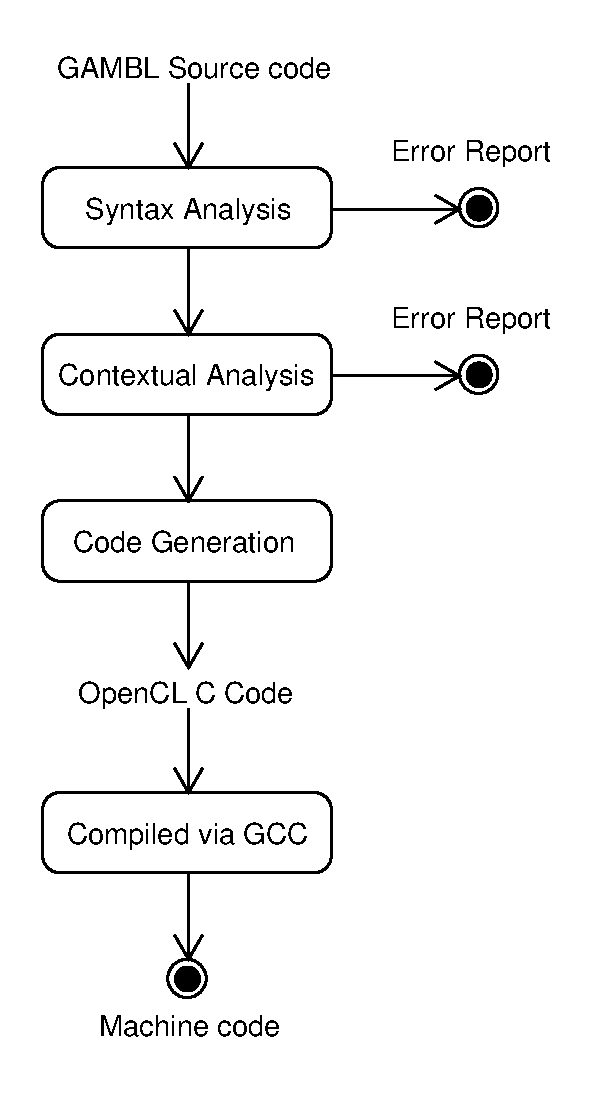
\includegraphics[width=0.5\textwidth]{figures/ClassDiagrams/CompilerDiagram.pdf}
\caption{State diagram showing the phases of the compiler when it takes \gls{gamble} source code and compiles it into machine code.}\label{fig:phases}
\end{figure}

\begin{figure}[t]
	\begin{sideways}
	%\fbox{
		\begin{minipage}{22.5cm}
			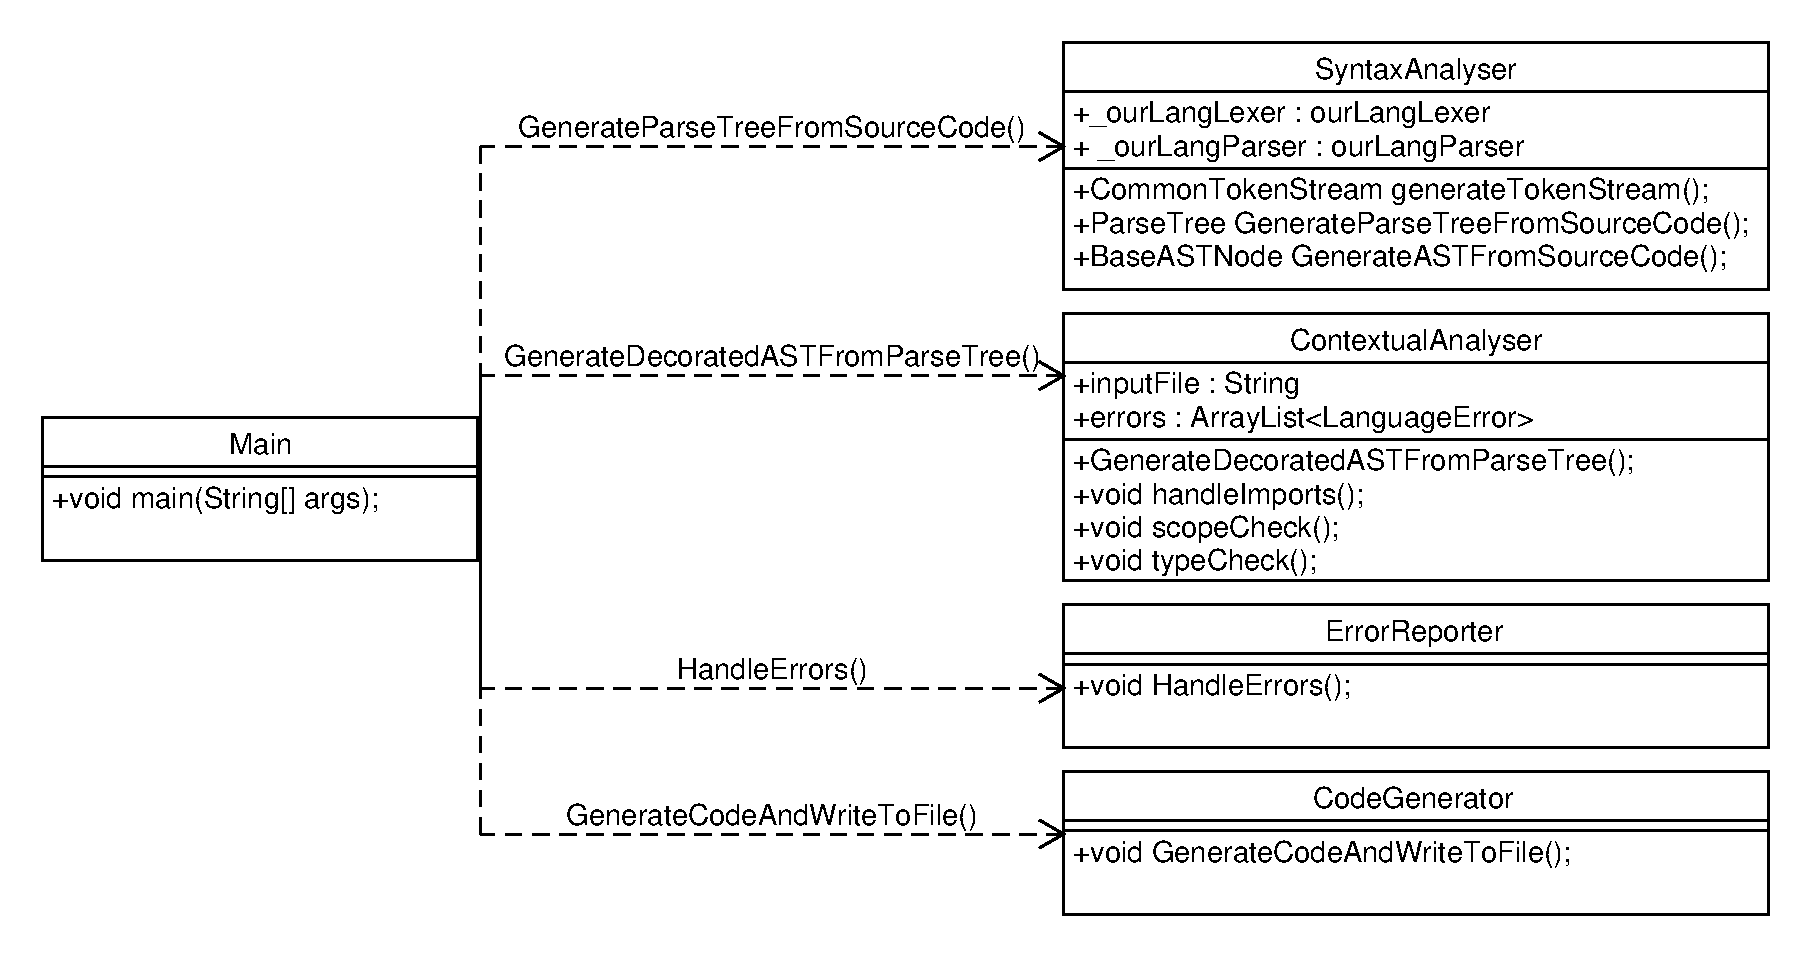
\includegraphics[height=0.42\textheight]{figures/ClassDiagrams/DiagramOfCallsFromMain.pdf}
		\end{minipage}
	%	}
	\end{sideways}
	\centering
	\caption{Diagram showing the structure of the compiler by showing the \texttt{main()} method's method calls. Arguments are omitted for simplicity}\label{fig:compilerOverview}
\end{figure}


%\begin{figure}[ht!]
%	\centering
%	\begin{tikzpicture}[node distance = 2.5cm]
%		\node (invi1) 		[invi,draw=none] {GAMBLE Source code};
%		\node (syntax) 		[blockz, below=0.6cm of invi1] {Syntax Analysis};
%		\node (contextual) 	[blockz, below of=syntax] {Contextual Analysis};
%		\node (codegen) 	[blockz, below of=contextual] {Code Generation};
%		\node (opencl) 		[invi,draw=none, below=0.6cm of codegen] {OpenCL C code};
%
%		\node (error1) 		[cloud, right=1cm of syntax] {Error reports};
%		\node (error2) 		[cloud, right=1cm of contextual] {Error reports};
%
%		\node (invi2) 		[invi,draw=none, below=0.4cm of syntax] {};
%		\node (ast) 		[invi,draw=none, right=-0.2cm of invi2] {Abstract Syntax Tree};
%
%		\node (invi3) 		[invi,draw=none, below=0.4cm of contextual] {};
%		\node (dast) 		[invi,draw=none, right=-0.5	cm of invi3] {Abstract Syntax Tree \& Symbol Table};
%
%		\draw [arrow] (invi1) -- (syntax);
%		\draw [arrow] (syntax) -- (contextual);
%		\draw [arrow] (contextual) -- (codegen);
%		\draw [arrow] (codegen) -- (opencl);
%		
%		\draw [arrow] (syntax) -- (error1);
%		\draw [arrow] (contextual) -- (error2);
%	\end{tikzpicture}
%	\caption{The phases of the compiler.}\label{fig:phases}
%\end{figure}
\clearpage

\label{SourceCodeAsTrees}
\todo{Write about Sourcecode as Trees, and why we do that.}

